\section{Results} \label{sec:results}

\Cref{table:results-selected-model} shows the average performance of the
selected in the \nameref{subsubsec:evaluatio-dataset} dataset. Performance is measured
with commonly used odometry and simultaneous localization and mapping metrics
as described in \cite{Measuring2019}. \Cref{fig:high-slip} shows its results on
an evaluation recording characterized by high slippage driving conditions using
two different devices.

\begin{table}
    \centering
    \begin{tabular}{|c|c|c|}
        \hline
                        & Mean ATE [m] & Mean RPE [m/s] \\ \hline
        All microphones & $1.02e-03$   & $5.10e-03$     \\
        \hline
    \end{tabular}
    \caption[Selected model average performance across evaluation recordings
        and devices]{Selected model average performance across all evaluation
        recordings and all devices. Average Trajectory Error (ATE) is computed
        between frames with a duration of 15 ms and Relative Pose Error (RPE)
        is computed using time windows 1s long.}
    \label{table:results-selected-model}
\end{table}


\begin{figure*}
    \centering
    \begin{tikzpicture} \node [anchor=south west] at (0,0) {
            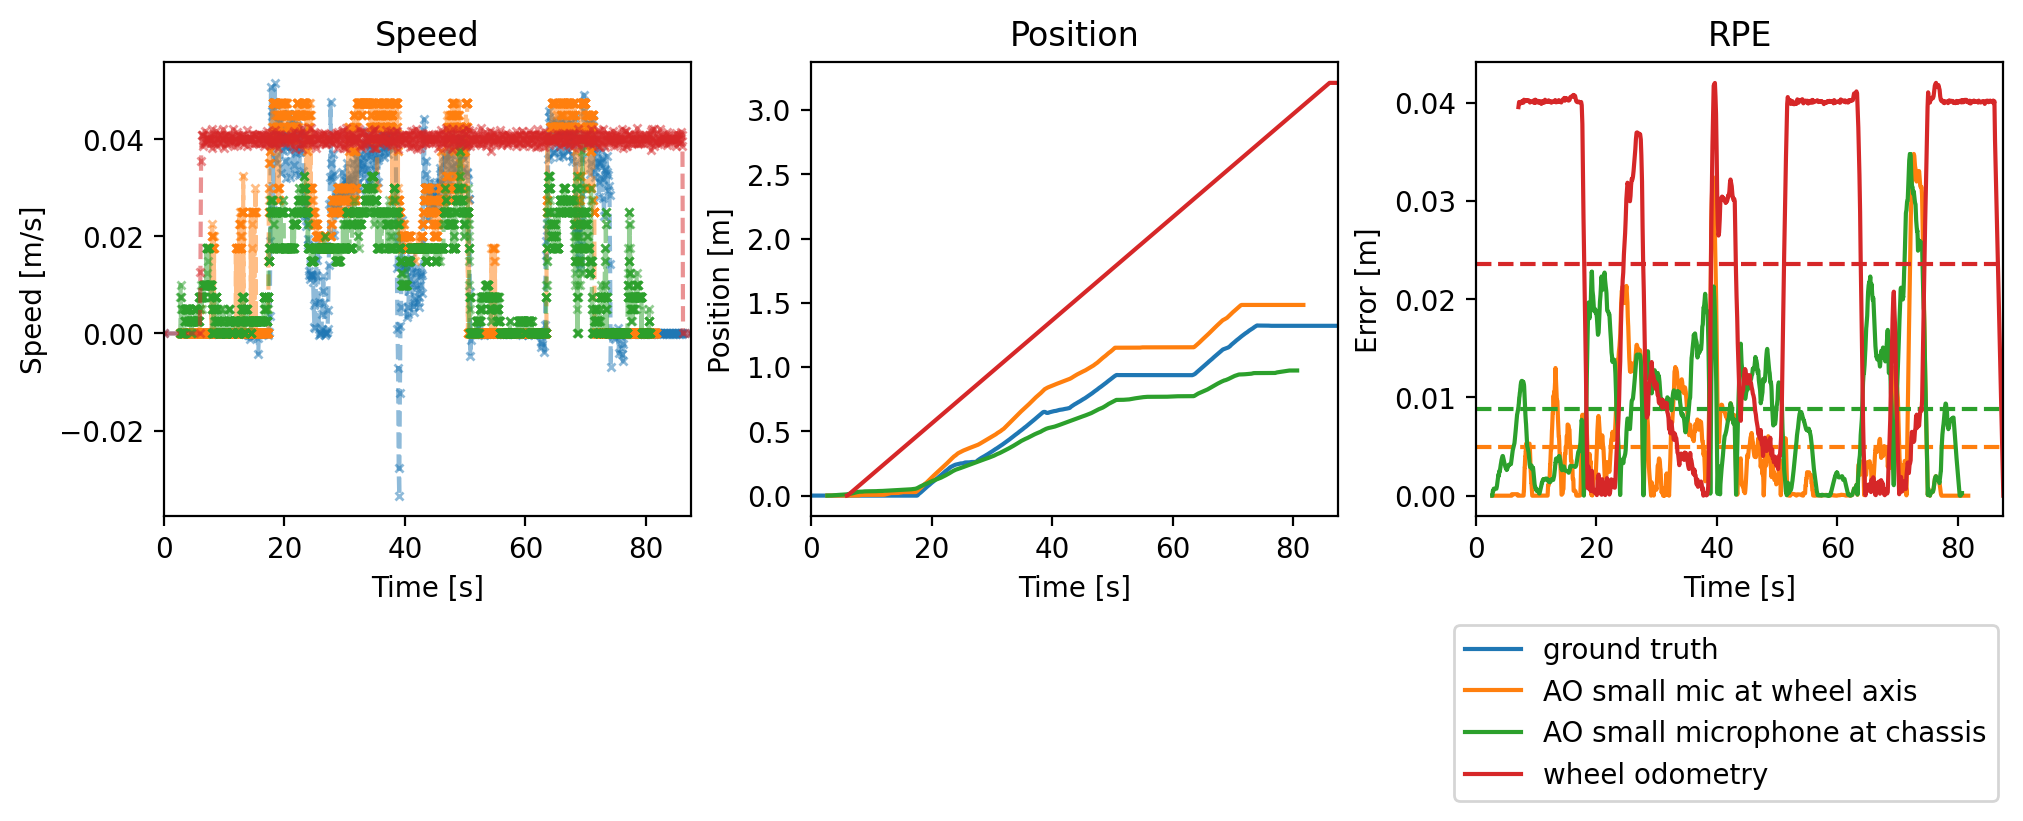
\includegraphics[width=.95\textwidth]{\subdir/high-slip.png}
        }; \node [anchor=south west, text width=.6\textwidth] at (0.5,0.5) {
            \caption{Selected model evaluated on a recording characterized by high
                slippage conditions using two different devices.}
            \label{fig:high-slip}
        }; \end{tikzpicture}
\end{figure*}

\subsection{Noise} One can see in \cref{fig:noise-effect} the behavior of the
selected model against white noise. Generally, white noise increases the value
of the estimated motion. Signal-to-Noise ratios of -20 dB impede the model to
recognize situations where the wheel is not moving.

\begin{figure*}
    \centering
    \begin{tikzpicture} \node [anchor=south west] at (0,0) {
            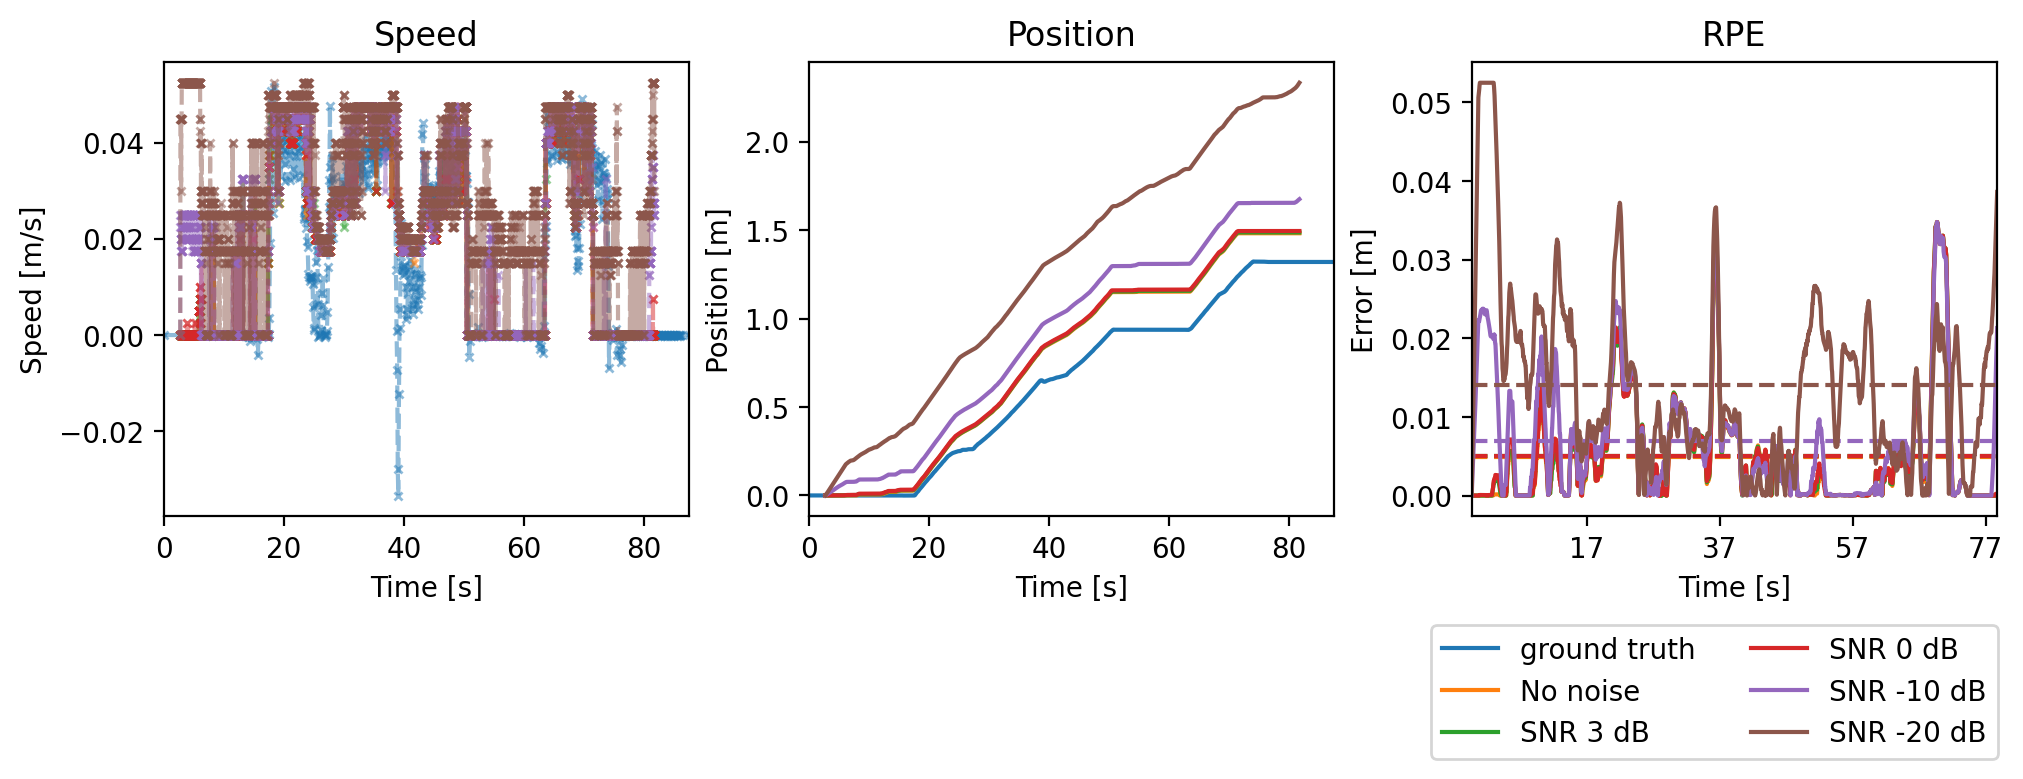
\includegraphics[width=.95\textwidth]{\subdir/noise-effect.png}
        }; \node [anchor=south west, text width=.6\textwidth] at (0.5,0.2) {
            \caption{Selected model evaluated on a
                recording with added white noise with varying signal-to-noise Ratio
                values.}
            \label{fig:noise-effect}
        }; \end{tikzpicture}
\end{figure*}

\subsection{Computational cost} Tests with the selected model on a CPU show
that the time to compute the feature extraction is a 40\% of the total time to
process a new frame, which is 2.03 ms on an Intel\textregistered{}
Core\texttrademark{} i7-9750H CPU at 2.60GHz. The prediction time takes up a
55\% of the total time while the remaining 5\% corresponds to loading the new
frame into memory. The system is able to run 7.5 times faster than real time on
this particular hardware. Using hardware acceleration with CUDA the total time
to process a new frame is slightly lower: 1.93 ms on a NVIDIA GeForce RTX 2060
GPU.

\subsection{Compared with other models} The selected model is evaluated against
two other odometry methods: Wheel odometry computed from the ground truth wheel
angular speed; and Visual SLAM using Intel\textregistered{}
RealSense\texttrademark{} Tracking Camera T265, which is based on visual
odometry. \Cref{fig:other-methods} is the evaluation in an ideal scenario for
all methods. It shows that the selected model can perform with an accuracy
comparable to state-of-the-art commercial visual-based methods in this
simplified scenario. \Cref{fig:VO-challenge} instead corresponds to a scenario
that is challenging for visual odometry. Dynamic objects are moved in the
camera field of view and lightning conditions are changed during the recording.
One can see in this evaluation that the vulnerabilities of audio-based odometry
and visual-based odometry do not overlap. Which makes Acoustic Odometry more
accurate in certain scenarios where the visual odometry vulnerabilities are
exploited.

\begin{figure*}
    \centering
    \begin{tikzpicture} \node [anchor=south west] at (0,0) {
            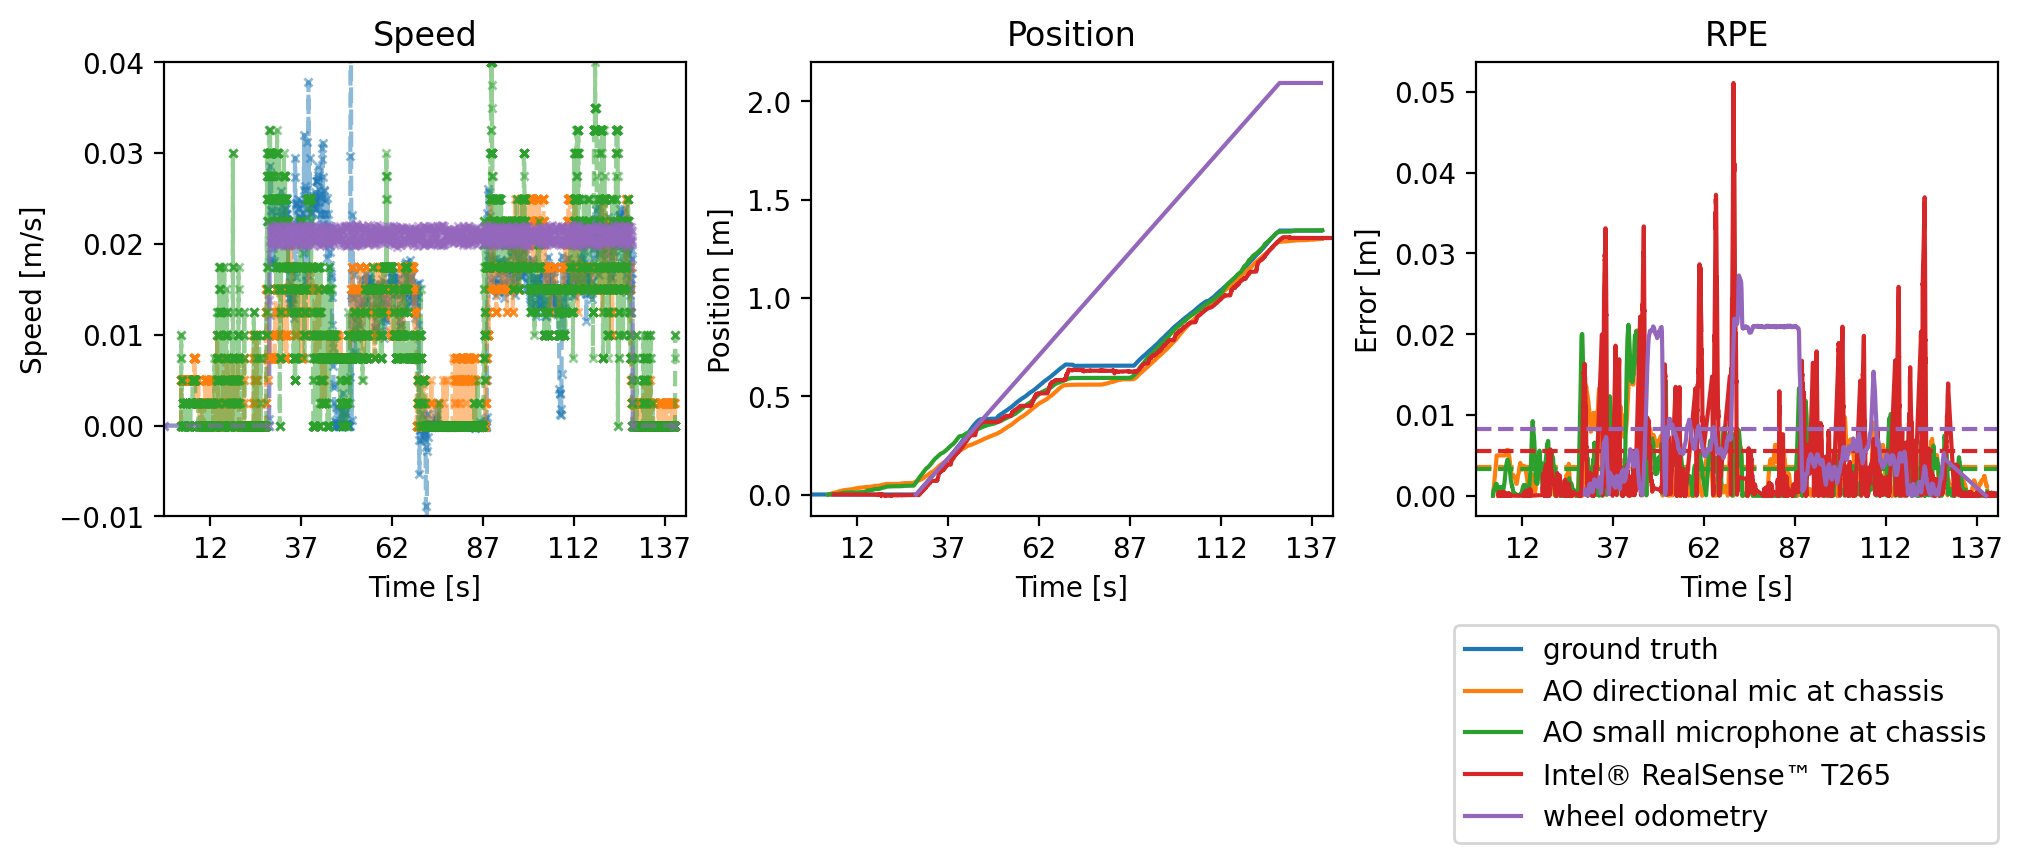
\includegraphics[width=.95\textwidth]{\subdir/other-methods.png}
        }; \node [anchor=south west, text width=.6\textwidth] at (0.5,0.5) {
            \caption{Selected model evaluated
                evaluated against Visual SLAM (based on visual odometry) and wheel
                odometry.}
            \label{fig:other-methods}
        }; \end{tikzpicture}
\end{figure*}

\begin{figure*}
    \centering
    \begin{tikzpicture} \node [anchor=south west] at (0,0) {
            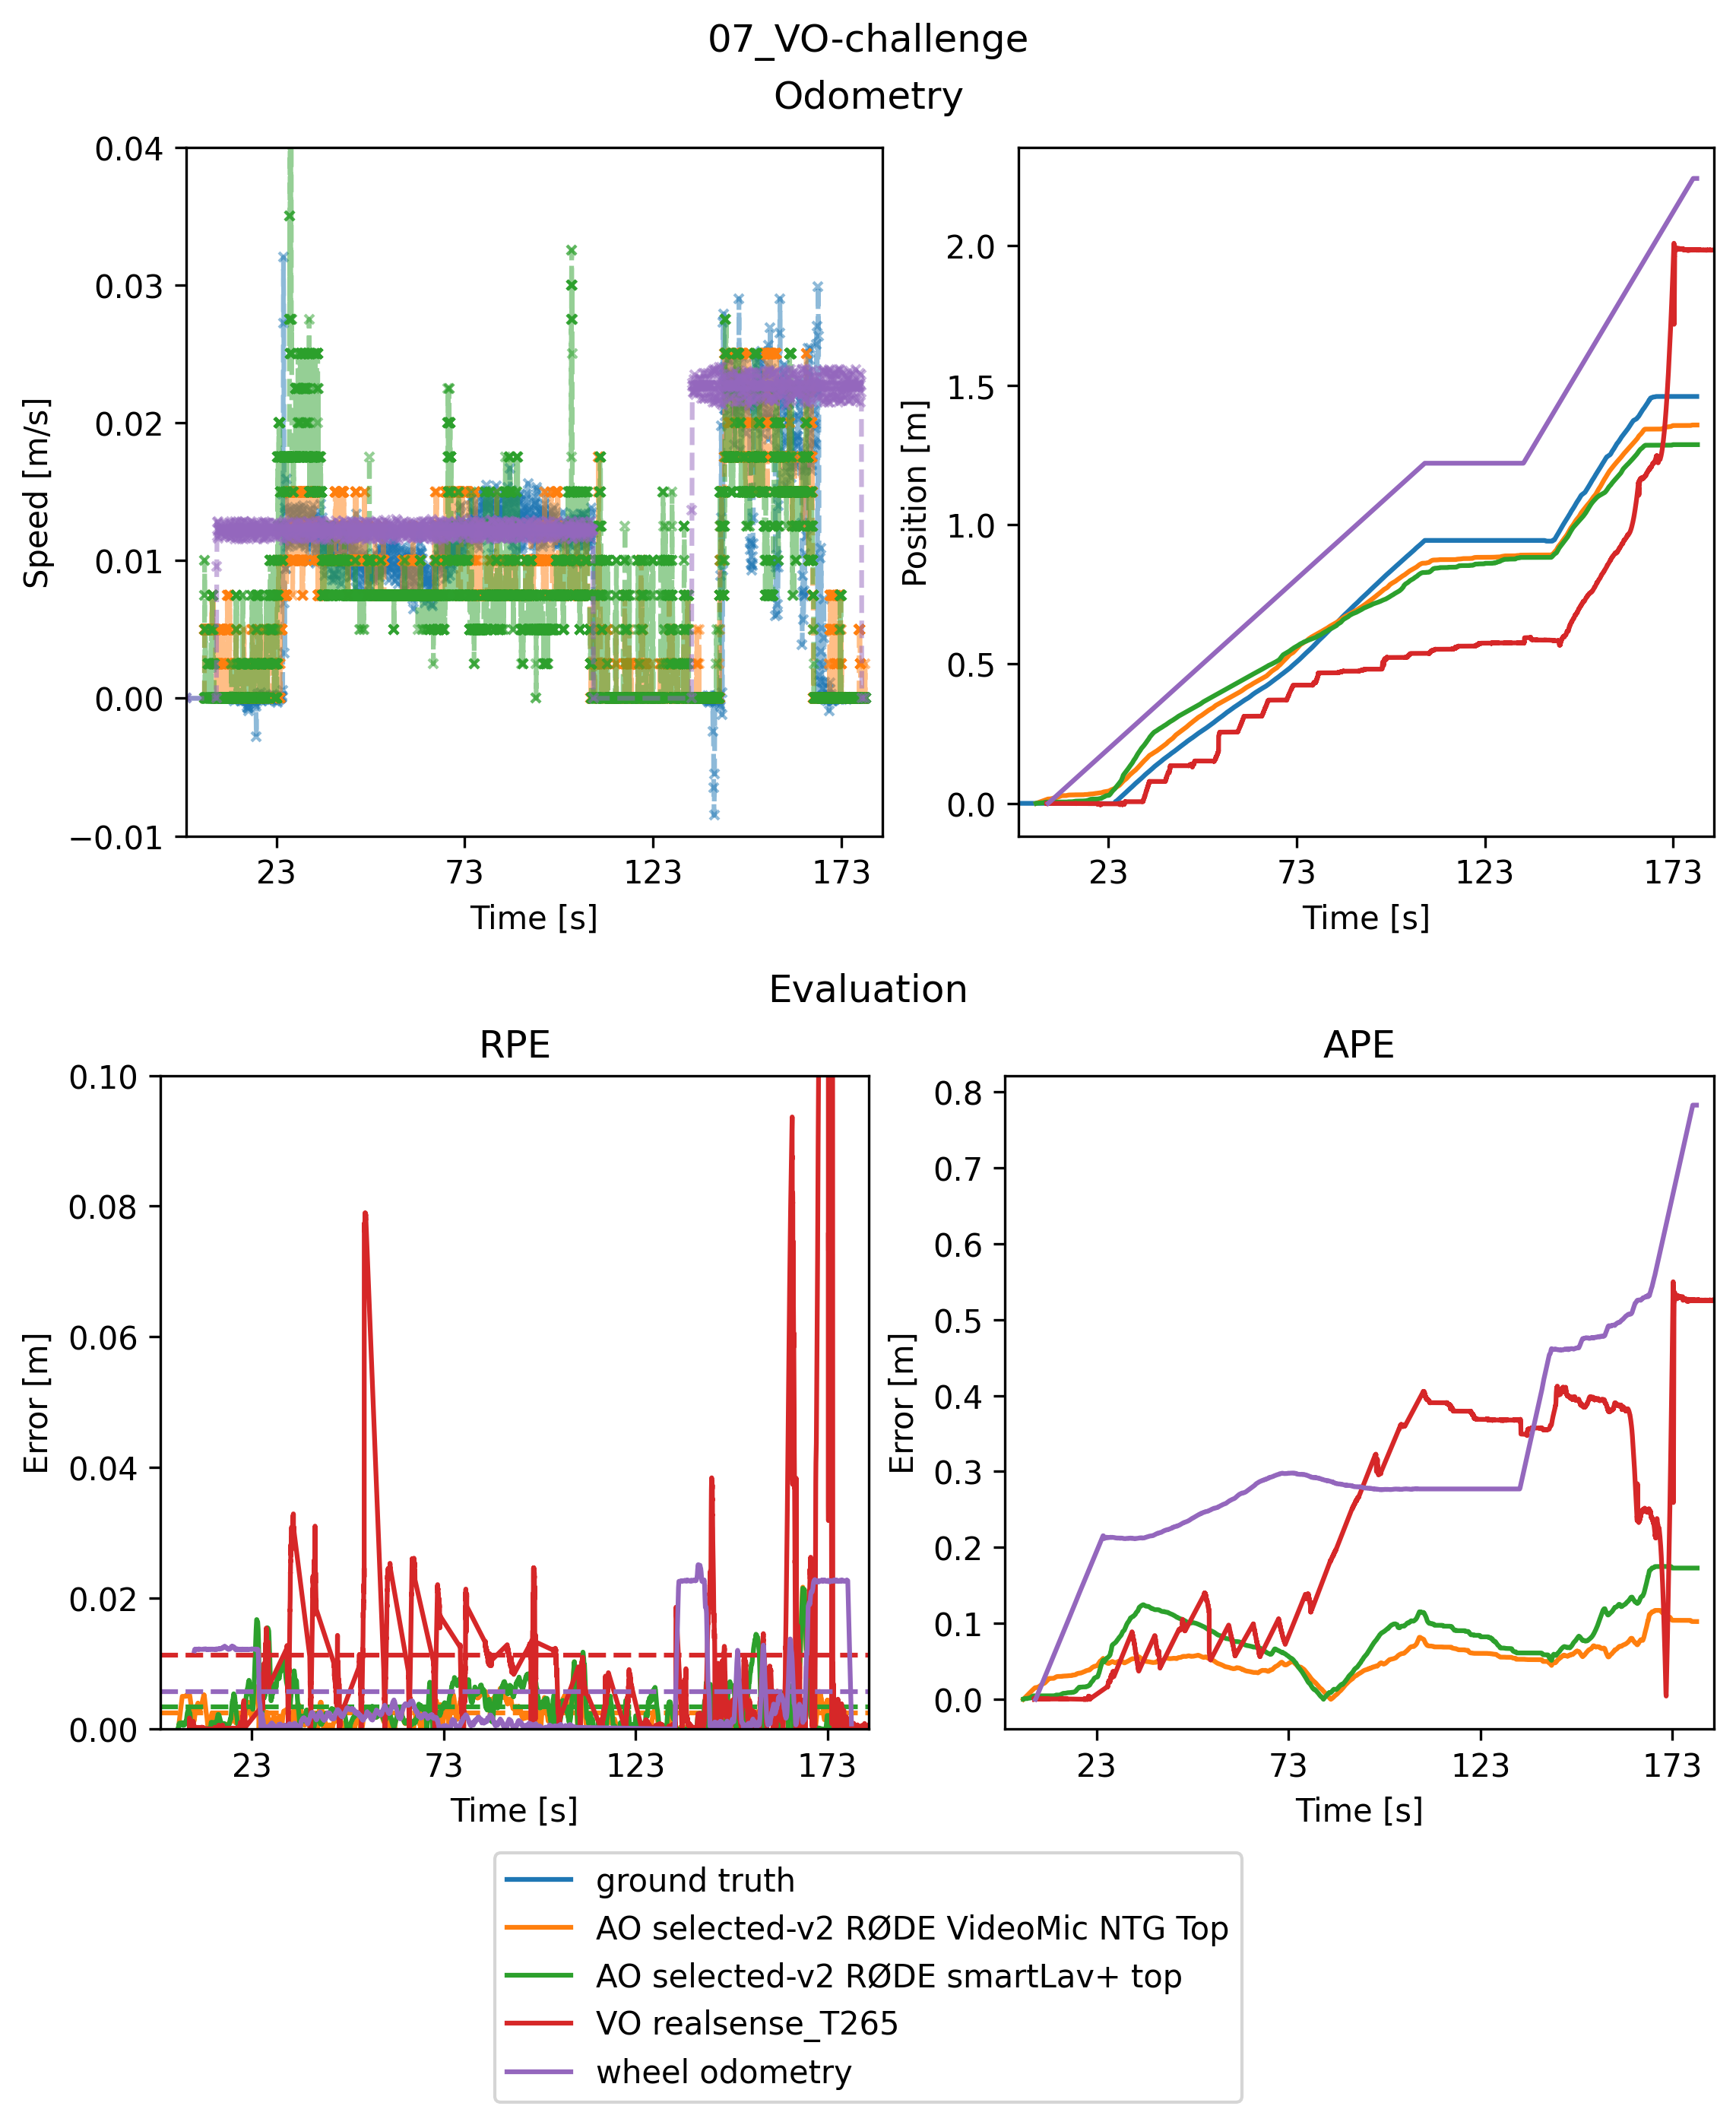
\includegraphics[width=.95\textwidth]{\subdir/VO-challenge.png}
        }; \node [anchor=south west, text width=.6\textwidth] at (0.5,0.1) {
            \caption{
                Selected model evaluated against Visual SLAM (based on visual odometry)
                in a scenario where visual odometry vulnerabilities are exploited:
                Dynamic objects are moved in the camera field of view and lightning
                conditions are changed during the recording.}
            \label{fig:VO-challenge}
        }; \end{tikzpicture}
\end{figure*}

\include*{\subdir/discussion}